% Vector replica of Fig. 2 of the submitted manuscript (Fig2.png, 1151 x 686 px); coordinates are the pixel
% positions of the original drawing (x right, y down), text and layout unchanged.
\documentclass[border=2pt]{standalone}
\usepackage[T1]{fontenc}\usepackage[scaled]{helvet}\renewcommand\familydefault{\sfdefault}
\usepackage{tikz}\usetikzlibrary{arrows.meta}
\definecolor{boxgreen}{RGB}{98,160,72}
\begin{document}
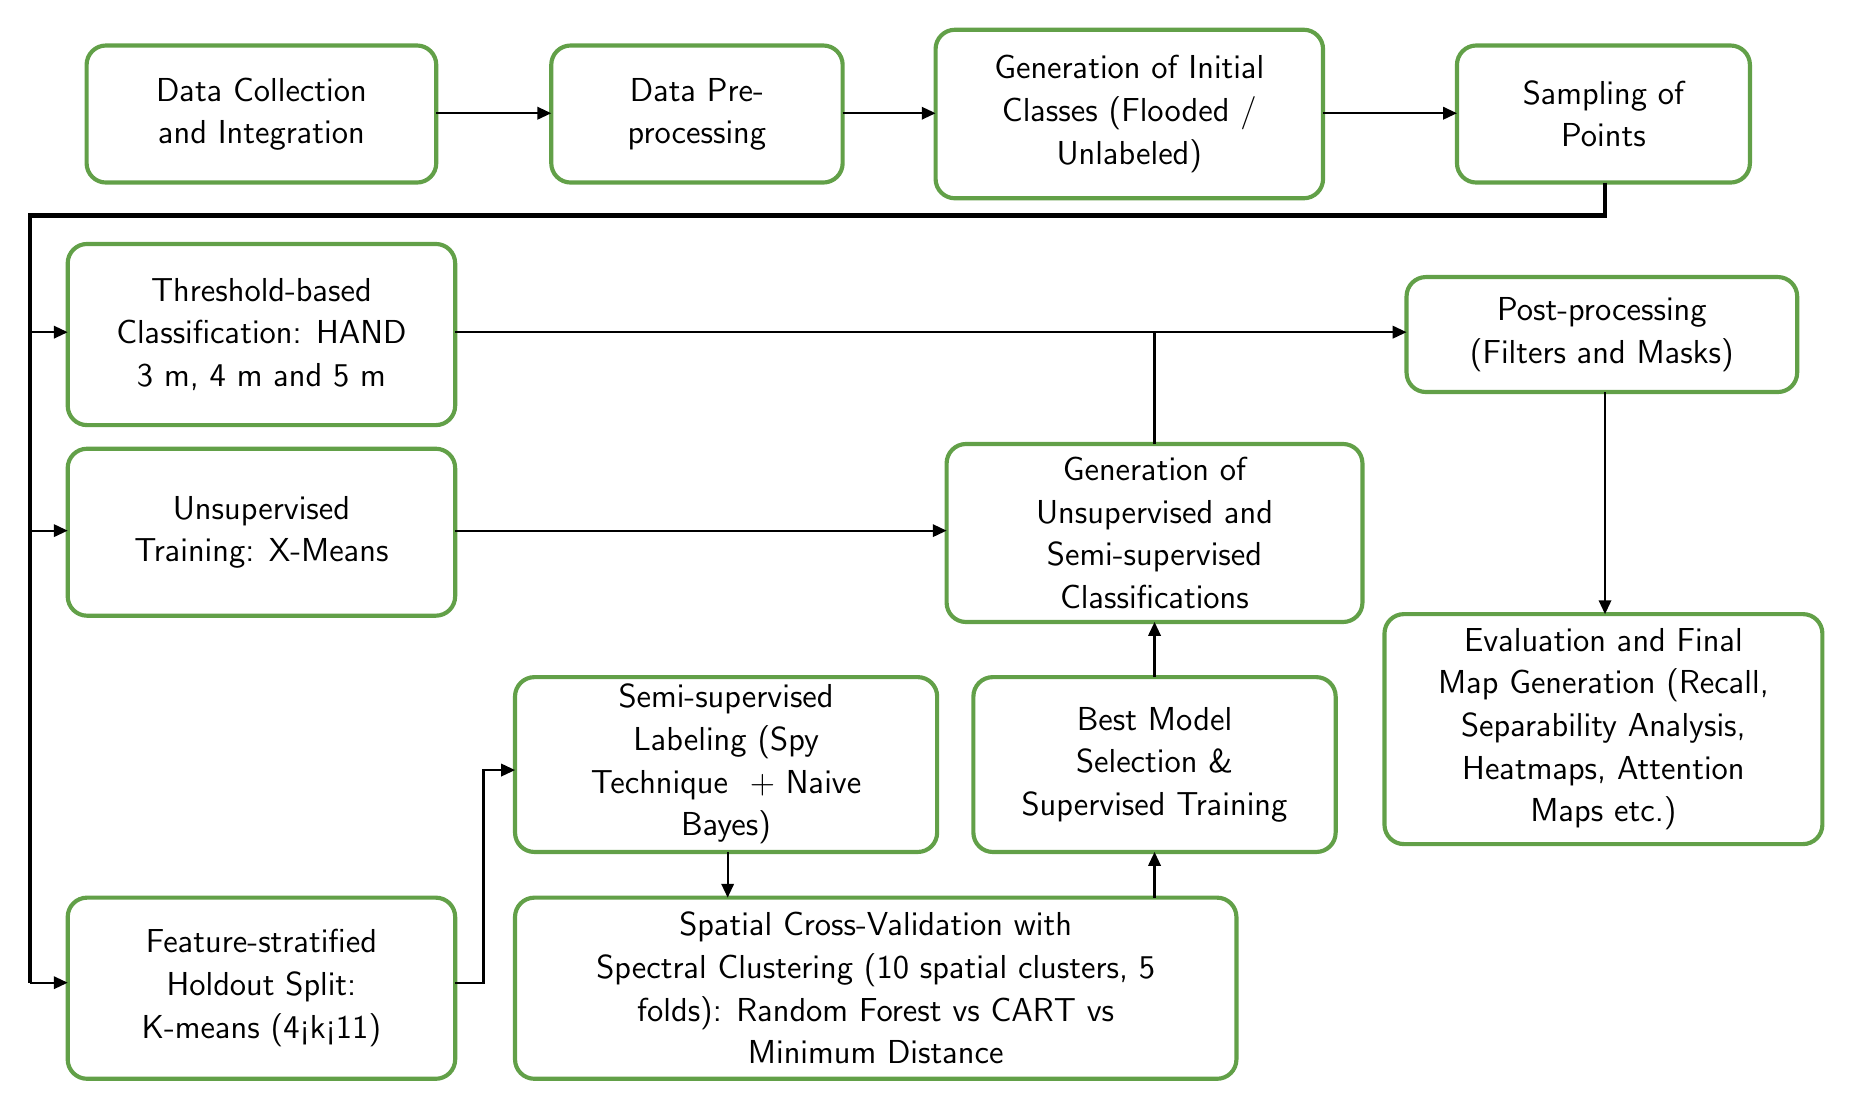
\begin{tikzpicture}[x=0.02cm, y=-0.02cm,
  bx/.style={draw=boxgreen, line width=1.5pt, rounded corners=7pt},
  tx/.style={align=center, font=\fontsize{13}{15.4}\selectfont, inner sep=0pt},
  arr/.style={-{Triangle[length=5pt,width=4.5pt]}, line width=0.75pt}]
\newcommand\B[5]{\draw[bx] (#1,#2) rectangle (#3,#4); \node[tx] at ({(#1+#3)/2},{(#2+#4)/2}) {#5};}
\B{48}{15}{270}{102}{Data Collection\\and Integration}
\B{343}{15}{528}{102}{Data Pre-\\processing}
\B{587}{5}{833}{112}{Generation of Initial\\Classes (Flooded /\\Unlabeled)}
\B{918}{15}{1104}{102}{Sampling of\\Points}
\B{36}{141}{282}{256}{Threshold-based\\Classification: HAND\\3 m, 4 m and 5 m}
\B{36}{271}{282}{377}{Unsupervised\\Training: X-Means}
\B{36}{556}{282}{671}{Feature-stratified\\Holdout Split:\\K-means (4<k<11)}
\B{594}{268}{858}{381}{Generation of\\Unsupervised and\\Semi-supervised\\Classifications}
\B{886}{162}{1134}{235}{Post-processing\\(Filters and Masks)}
\B{872}{376}{1150}{522}{Evaluation and Final\\Map Generation (Recall,\\Separability Analysis,\\Heatmaps, Attention\\Maps etc.)}
\B{320}{416}{588}{527}{Semi-supervised\\Labeling (Spy\\Technique \ + Naive\\Bayes)}
\B{611}{416}{841}{527}{Best Model\\Selection \&\\Supervised Training}
\B{320}{556}{778}{671}{Spatial Cross-Validation with\\Spectral Clustering (10 spatial clusters, 5\\folds): Random Forest vs CART vs\\Minimum Distance}
\draw[arr] (270,58) -- (343,58);
\draw[arr] (528,58) -- (587,58);
\draw[arr] (833,58) -- (918,58);
\draw[line width=1.6pt] (1012,102) -- (1012,123) -- (12,123) -- (12,610);
\draw[arr] (12,197) -- (36,197);
\draw[arr] (12,323) -- (36,323);
\draw[arr] (12,610) -- (36,610);
\draw[arr] (282,197) -- (886,197);
\draw[line width=0.75pt] (726,268) -- (726,197);
\draw[arr] (282,323) -- (594,323);
\draw[arr] (1012,235) -- (1012,376);
\draw[arr] (282,610) -- (300,610) -- (300,475) -- (320,475);
\draw[arr] (455,527) -- (455,556);
\draw[arr] (726,556) -- (726,527);
\draw[arr] (726,416) -- (726,381);
\end{tikzpicture}
\end{document}
